\documentclass[11pt,notitlepage]{article}
\usepackage[a4paper, margin={2cm, 2.2cm}]{geometry}
\usepackage[a-2b]{pdfx}[2018/12/22]
\usepackage{alltt, fancyvrb, url}
\usepackage{graphicx}
\usepackage[utf8]{inputenc}
\usepackage{float}
\usepackage{hyperref}
\usepackage{subcaption}
\usepackage{numprint}
\usepackage{slashbox}
\usepackage{pgfplots}
\usepackage{amsmath}
\usepackage{lipsum}
\usepackage{tikz}
\pgfplotsset{compat=1.9,
            tick label style={font=\tiny},
            label style={font=\tiny}}

% Questo commentalo se vuoi scrivere in inglese.
\usepackage[italian]{babel}

\usepackage[italian]{cleveref}

\title{Programmazione concorrente e distribuita \\ Assignment 01}

\author{
    \href{mailto:nicolo.guerra@studio.unibo.it}{Nicolò Guerra, matricola 0001179571} \\
    \href{mailto:filippo.casadei9@studio.unibo.it}{Filippo Casadei, matricola 0001179572} \\
    \href{mailto:emma.leonardi2@studio.unibo.it}{Emma Leonardi, matricola 0001193227}
    }
\date{\today}

\begin{document}
\maketitle
\renewcommand{\thesection}{\arabic{section}}
\section{Analisi del problema}
Il problema riguarda la parallelizzazione dell'algoritmo Boids. La parte su cui si è concentrata la parallelizzazione è quella del calcolo delle velocità e delle posizioni dei 
boids. Dato che il calcolo delle posizioni richiede la lettura delle velocità è necessario un qualche tipo di sincronizzazione tra le due attività per evitare corse critiche.
Inoltre l'aggiornamento della view richiede la sola lettura delle posizioni dei boid, perciò può lavorare in parallelo con l'aggiornamento delle velocità ma non delle posizioni dei boid.
Attualmente la versione sequenziale aggiorna i boid uno di seguito all'altro senza effettuare un istantanea del modello all'inizio di ogni iterazione. Questo comporta che i boid,
il cui aggiornamento si basa sui valori delle posizioni e velocità dei boid vicini, possano basare i propri dati su altri in parte aggiornati e in parte no. Questo non è un grosso
problema per la versione sequenziale mentre nella versione concorrente potrebbe portare a risultati non corretti, o in caso di sincronizzazione errata a deadlock, ma anche nel caso di
sincronizzazione corretta comporterebbe lunghi periodi di attesa e un basso livello di parallelismo, per questo si è deciso di lavorare ad ogni iterazione su una copia del model che ne 
rappresenta l'istantanea all'inizio del ciclo corrente.
Le soluzioni proposte sono tre diverse implementazioni, ognuna delle quali sfrutta un diverso approccio di programmazione concorrente. 
Le tre soluzioni sono: 
\begin{itemize}
    \item \textbf{Platform Threads}: utilizza i platform threads del sistema operativo per parallelizzare l'algoritmo.
    \item \textbf{Task-based}: utilizza l'approccio basato su task e sulla API Java Executor Framework.
    \item \textbf{Virtual Threads}: utilizza i virtual threads di Java per parallelizzare l'algoritmo.
\end{itemize}

\section{Introduzione}
È stata implementata una classe base astratta \textsf{BoidsSimulator} che contiene il model, la view, i metodi per fermare e avviare la simulazione e il metodo astratto 
\textsf{runSimulation()} che conterrà il main loop della simulazione e che deve essere implementato dalle tre classi derivate.

Contiene inoltre un oggetto di classe \textsf{SimulatorStateMonitor}, che è stata implementata con tutti metodi \textsf{synchronized} per contenere lo stato della simulazione
e fornire i metodi per fermarla e avviarla.

\section{Platform Threads}
Per la soluzione basata su threads si è deciso di utilizzare un numero di thread pari al numero di processori della macchina aumentato di 1. La lista dei Boid è stata
quindi partizionata in un numero di sotto-liste pari al numero di thread, in modo che ogni thread possa lavorare su una sotto-lista di Boid.
Dato che ogni thread ha bisogno di scrivere la posizione e la velocità dei Boids su cui lavora e di leggere quelle dei Boids vicini, si è deciso per evitare meccanismi di 
sincronizzazione che avrebbero portato a rallentamenti importanti di lavorare su copie del model e di sincronizzare gli aggiornamenti al model principale solo alla fine di ogni
iterazione.

L'iterazione inizia perciò con i thread bloccati da una barriera in attesa che il main assegni a ciascuno una copia del model. Il main sblocca poi la barrier e ogni
thread esegue l'aggiornamento delle velocità concorrentemente al disegno della view da parte del main thread (le velocità non vengono lette durante l'aggiornamento della view).
A questo punto i thread si bloccano nuovamente su una barriera in modo che possano proseguire solo quando tutti hanno aggiornato le velocità dei propri boid e il main ha aggiornato
la view. Aggiornano quindi le posizioni dei Boids e si bloccano nuovamente sulla barriera. A questo punto il main thread controlla se la simulazione deve essere fermata per un comando
di pause o stop e se non è così sblocca i thread per l'iterazione successiva.

In caso di stop il main thread esegue l'interrupt di tutti i worker threads che terminano l'esecuzione e il main thread termina la simulazione facendo il join di tutti i worker.

\begin{figure}[H]
    \centering
    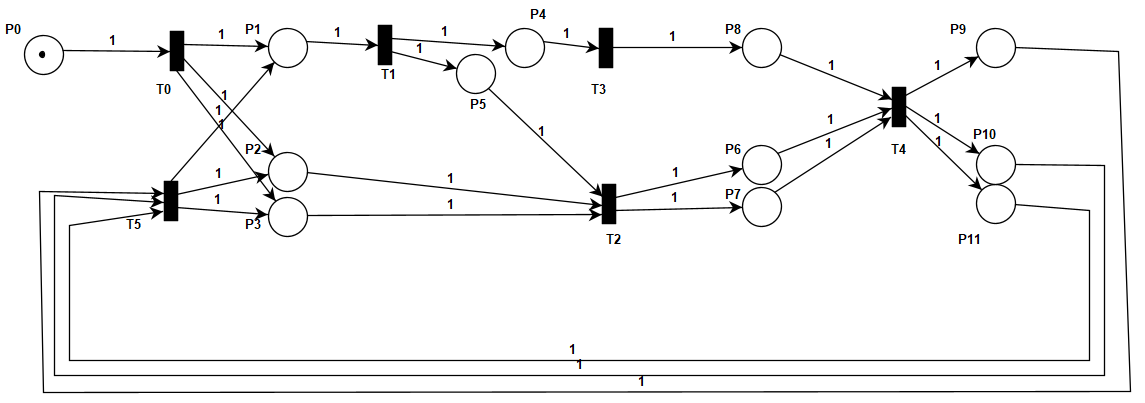
\includegraphics[width=\textwidth]{Petri net 1.png}
    \caption{Petri net della soluzione Platform Threads con 2 worker.}
    \label{fig:platform-threads-diagram}
\end{figure}

\begin{table}[H]
    \centering
    \begin{tabular}{|c|l|}
        \hline
        \textbf{Stato/Transizione} & \multicolumn{1}{c|}{\textbf{Descrizione}} \\
        \hline
        \rule{0pt}{2.5ex} \textbf{P0} & \multicolumn{1}{c|}{Il main all'inizio.} \\[0.5ex]
        \hline
        \rule{0pt}{2.5ex} \textbf{T0} & \multicolumn{1}{c|}{L'azione di creazione dei thread.} \\[0.5ex]
        \hline
        \rule{0pt}{2.5ex} \textbf{P1} & \multicolumn{1}{c|}{Il main dopo aver creato i thread.} \\[0.5ex]
        \hline
        \rule{0pt}{2.5ex} \textbf{P2} e \textbf{P3} & \multicolumn{1}{c|}{2 worker thread appena creati.} \\[0.5ex]
        \hline
        \rule{0pt}{2.5ex} \textbf{T1} & \multicolumn{1}{c|}{L'azione di assegnazione del model ai thread.} \\[0.5ex]
        \hline
        \rule{0pt}{2.5ex} \textbf{P4} & \multicolumn{1}{c|}{Il main dopo aver assegnato il model ai thread.} \\[0.5ex]
        \hline
        \rule{0pt}{2.5ex} \textbf{P5} & \multicolumn{1}{c|}{Il main dopo aver sbloccato i thread.} \\[0.5ex]
        \hline
        \rule{0pt}{2.5ex} \textbf{T2} & \multicolumn{1}{c|}{L'azione di aggiornamento delle velocità dei boids.} \\[0.5ex]
        \hline
        \rule{0pt}{2.5ex} \textbf{P6} e \textbf{P7} & \multicolumn{1}{c|}{I worker thread dopo aver aggiornato le velocità dei boids.} \\[0.5ex]
        \hline
        \rule{0pt}{2.5ex} \textbf{T3} & \multicolumn{1}{c|}{L'azione di aggiornamento della view.} \\[0.5ex]
        \hline
        \rule{0pt}{2.5ex} \textbf{P8} & \multicolumn{1}{c|}{Il main dopo aver aggiornato la view.} \\[0.5ex]
        \hline
        \rule{0pt}{2.5ex} \textbf{T4} & \multicolumn{1}{c|}{L'azione di aggiornamento delle posizioni dei boids.} \\[0.5ex]
        \hline
        \rule{0pt}{2.5ex} \textbf{P9} & \multicolumn{1}{c|}{Il main dopo che i thread hanno aggiornato le posizioni.} \\[0.5ex]
        \hline
        \rule{0pt}{2.5ex} \textbf{P10} e \textbf{P11} & \multicolumn{1}{c|}{I worker thread dopo aver aggiornato le posizioni dei boids.} \\[0.5ex]
        \hline
        \rule{0pt}{2.5ex} \textbf{T5} & \multicolumn{1}{c|}{L'azione di sblocco dei thread per l'iterazione successiva.} \\[0.5ex]
        \hline
    \end{tabular}
    \caption{Descrizione degli stati e delle transizioni nella Petri Net \ref{fig:platform-threads-diagram}.}
    \label{tab:petri-net-description}
\end{table}

\newpage
\section{Task-based}
La soluzione task-based è stata implementata utilizzando l'API Java Executor Framework. All'inizio della funzione \textsf{runSimulation()} viene creato un 
\textsf{ExecutorService} di tipo \textsf{FixedThreadPool} con un numero di thread pari al numero di processori della macchina aumentato di 1.
Il main si occupa di creare i task di aggiornamento delle velocity e di sottometterli all'\textsf{ExecutorService}, ne attende quindi il completamento 
chiamando il get sull'oggetto \textsf{Future} di ogni task. Mette quindi in coda i task di aggiornamento delle posizioni e attende il completamento anche di 
questi. Il main aggiorna quindi la view, controlla se la simulazione deve essere fermata o messa in pausa e in caso negativo procede con l'iterazione successiva.
Nel caso in cui la simulazione debba essere fermata il main chiama il metodo \textsf{shutdown()} sull'\textsf{ExecutorService} e termina la simulazione.

\section{Virtual Threads}
La soluzione basata su virtual threads è stata implementata utilizzando un singolo virtual thread per ogni boid. Questo è possibile
grazie al fatto che i virtual threads sono molto leggeri e possono essere creati in un numero molto maggiore rispetto ai platform threads.
Il main thread crea quindi un virtual thread per ogni boid e lo esegue. Il loop si svolge in modo simile alla soluzione basata su platform threads con gli stessi punti
di sincronizzazione ottenuta attraverso una barriera.

\section{Dettagli implementativi}
\subsection{SimulatorStateMonitor}
La classe \textsf{SimulatorStateMonitor} contiene lo stato della simulazione e i metodi per fermarla e avviarla. Tutti i metodi sono \textsf{synchronized} per evitare
corse critiche. Quando viene chiamato uno tra i due metodi \textsf{resume} o \textsf{stop} oltre all'aggiornamento dei flag viene chiamato \textsf{notifyAll} in modo
che i thread in attesa su questo oggetto possano riprendere l'esecuzione.

\subsection{SimpleBarrier}
La classe \textsf{SimpleBarrier} implementa una semplice barriera per la sincronizzazione fra thread. Contiene una \textsf{Condition} su cui i threads che chiamano
\textsf{await} si mettono in attesa dopo aver incrementato un contatore, quando il contatore raggiunge il numero di threads che devono passare la barriera, il 
thread che ha incrementato il contatore per ultimo lo resetta e sveglia tutti chiamando \textsf{signalAll} sull'oggetto \textsf{Condition}.
La classe è resa thread-safe mediante un \textsf{ReentrantLock}.

\section{Verifica JPF della versione Platform Threads}
Una prima verifica della versione Platform Threads effettuata con Java Path Finder ha mostrato la presenza di un possibile deadlock dovuto all'assenza di un blocco try-finally
nel metodo \textsf{await} della \textsf{SimpleBarrier}. Questo comportava un rischio di deadlock in caso di interruzione del thread quando questo era in attesa sulla condition, perché 
lanciando eccezione non avrebbe mai rilasciato il lock.
Risolto questo problema l'esecuzione di Java Path Finder non ha trovato ulteriori problemi.
Sono riportate le statistiche di esecuzione della verifica:
\begin{verbatim}
states:             new=32414479, visited=63876782, backtracked=96291261, end=10
search:             maxDepth=1606, constraints=0
choice generators:  thread=32414478 (signal=0, lock=676529, sharedRef=28821190, 
                    threadApi=180, reschedule=2789380), data=0
heap:               new=7400851, released=8790839, maxLive=1369, gcCycles=93268219
instructions:       1574428373
max memory:         1708MB
loaded code:        classes=188, methods=3966
\end{verbatim}

\section{Performance}

\subsection{Misurazioni}

Per valutare le prestazioni delle varie implementazioni si è utilizzata come metrica gli FPS (Frame per second) medi dell'esecuzione di 500 iterazioni di aggiornamento.
Ogni versione è stata fatta girare più volte con un diverso numero di boids e, senza contare la versione seriale, utilizzando tutti i core disponibili.
Nel grafico \ref{fig:performance} sono riportati gli FPS medi in base al numero di boids per ogni versione:

\begin{figure}[H]
    \centering
    \begin{tikzpicture}
        \begin{axis}[
            width=16cm, height=10cm,
            xlabel={Numero di Boids},
            ylabel={FPS medi},
            legend pos=north east,
            grid=both,
            xtick=data,
            ymin=0,
            ymax=350,
            ymajorgrids=true,
            xmajorgrids=true,
            grid style=dashed,
            scaled x ticks=false,
        ]
        % Serial Simulation
        \addplot[
            color=red,
            mark=square,
            thick
        ] coordinates {
            (3000, 32.066)
            (5000, 11.540)
            (8000, 4.625)
            (10000, 2.594)
            (12000, 1.116)
            (14000, 1.078)
        };
        \addlegendentry{Serial Simulation}

        % Platform Threads Simulation
        \addplot[
            color=blue,
            mark=triangle,
            thick
        ] coordinates {
            (3000, 260.960)
            (5000, 83.514)
            (8000, 48.723)
            (10000, 32.624)
            (12000, 20.029)
            (14000, 7.000)
        };
        \addlegendentry{Platform Threads Simulation}

        % Task-Based Simulation
        \addplot[
            color=green,
            mark=o,
            thick
        ] coordinates {
            (3000, 333.111)
            (5000, 111.111)
            (8000, 63.468)
            (10000, 40.727)
            (12000, 24.397)
            (14000, 8.452)
        };
        \addlegendentry{Task-Based Simulation}

        % Virtual Threads Simulation
        \addplot[
            color=purple,
            mark=diamond,
            thick
        ] coordinates {
            (3000, 277.932)
            (5000, 83.486)
            (8000, 48.454)
            (10000, 31.996)
            (12000, 19.908)
            (14000, 7.007)
        };
        \addlegendentry{Virtual Threads Simulation}

        \end{axis}
    \end{tikzpicture}
    \caption{FPS medi in base al numero di Boids.}
    \label{fig:performance}
\end{figure}

\subsection{Scalabilità}
Le varie implementazioni risultano scalabili dato che, aumentando il numero di core disponibili, il programma riesce a gestire un numero sempre maggiore di boids senza far calare le prestazioni.

Per misurare la scalabilità sono stati eseguiti dei test variando il numero di core utilizzati, seguono le configurazioni testate e per ogni versione la quantità massima di Boids che permette al programma di restare a 25 FPS medi
sempre su 500 iterazioni. I risultati sono mostrati in tabella \ref{tab:boids-performance} e nel grafico \ref{fig:scalability-graph}.

\begin{table}[H]
    \centering
    \begin{tabular}{|c|c|c|}
        \hline
        \textbf{Numero di Core} & \textbf{Platform Threads (Boids)} & \textbf{Task-Based (Boids)} \\
        \hline
        28 & 11500 & 12500 \\
        \hline
        16 & 9800 & 10200 \\
        \hline
        8  & 8700 & 8900 \\
        \hline
        4  & 7300 & 7500 \\
        \hline
        2  & 5000 & 5500 \\
        \hline
    \end{tabular}
    \caption{Numero massimo di Boids a 25 FPS medi in base al numero di core.}
    \label{tab:boids-performance}
\end{table}

\begin{figure}[H]
    \centering
    \begin{tikzpicture}
        \begin{axis}[
            width=16cm, height=10cm,
            xlabel={Numero di Core},
            ylabel={Numero massimo di Boids a 25 FPS medi},
            legend pos=north west,
            grid=both,
            xtick=data,
            ymin=0,
            ymajorgrids=true,
            xmajorgrids=true,
            grid style=dashed,
            scaled y ticks=false,
            scaled x ticks=false,
        ]
        % Platform Threads
        \addplot[
            color=blue,
            mark=square,
            thick
        ] coordinates {
            (2, 5000)
            (4, 7300)
            (8, 8700)
            (16, 9800)
            (28, 11500)
        };
        \addlegendentry{Platform Threads}

        % Task-Based
        \addplot[
            color=green,
            mark=triangle,
            thick
        ] coordinates {
            (2, 5500)
            (4, 7500)
            (8, 8900)
            (16, 10200)
            (28, 12500)
        };
        \addlegendentry{Task-Based}
        \end{axis}
    \end{tikzpicture}
    \caption{Numero massimo di Boids a 25 FPS medi in base al numero di core disponibili.}
    \label{fig:scalability-graph}
\end{figure}

Lo scaling, come si può osservare dal grafico \ref{fig:scalability-graph}, non è lineare, questo è dovuto alla porzione non parallelizzabile del programma.

\section{Conclusioni}

La versione seriale scende sotto i 25 FPS già a 5000 boids, mentre le versioni concorrenti riescono a mantenere un buon numero di FPS medi anche con 10000-12000 Boids.
Fra le versioni concorrenti quella che si dimostra più performante è la versione Task-Based, che riesce a mantenere un numero di FPS medi seppur di poco maggiore rispetto alle altre due.
Questo è probabilmente dovuto al fatto che lavorando a più alto livello si lascia lo spazio alle implementazioni sottostanti di operare ottimizzazioni anche a livello di VM.
Si attestano circa sulle stesse prestazioni le versioni Platform Thread e Virtual Thread, il che dimostra quanto i virtual thread risultino più leggeri rispetto ai thread del sistema operativo, dato che ne vengono
creati uno per boid e non si nota un calo di prestazioni rispetto alla versione Platform Thread.

\end{document}
